\chapter{Fundamentals of Surgery Theory}\label{chap:construction}

\begin{flushleft}
	\textsl{}\\
	\rule[0pt]{15em}{0.5pt}\\
	\textsl{-- }
	\vspace{2em}
\end{flushleft}

Within seven years of Milnor's 1956 announcement \cite{milnor1956manifolds} of his discovery of an exotic smooth structure on the $7$-sphere, the smooth structures on spheres of all but some tricky dimensions were completely classified  -- at the very least the problem was reduced to several better understood problems (see \cite{milnor1960homotopyspheres} and \cite{milnor1963groups}).
Such a quick turnaround is uncommon in mathematics, and this period of rapid growth starting in the late 1950s up until the late 1970s has been referred to as the ``golden age of topology''.
One of the great discoveries which emerged from this flurry of research was \defn{surgery theory}, a collection of techniques used to alter the topology of a manifold in a controlled way. This is usually done with respect to a loose notion of equivalence like cobordism -- for instance, we might use surgery to construct the simplest representative of a particular cobordism class.

In \cref{chap:introduction}, we saw how the problem of constructing and classifying exotic spheres can be reduced to a problem in cobordism, at least in dimensions $\geq 5$. This reduction gives us a foothold into the seemingly intractible problem of classifying smooth structures on spheres, but the resulting cobordism problem is still very hard.
Part of the difficulty is the almost complete lack of geometric information on homotopy spheres. A homotopy-sphere is, by definition, homotopy equivalent to a sphere, and so most of our usual invariants don't give us any useful information. However, there is a clever remedy to this issue. A useful principle in geometric topology is that the structure of manifolds is tightly coupled to the structure of manifolds which they bound.  The idea of studying $n$-dimensional topology by means of $(n+1)$-dimension topology with boundary is ubiquitous across mathematics and physics. \todo{mention cobordism, geometric invariants in later section, chern-simons theory}

\begin{definition}
	A manifold $W$ with boundary $X$ is said to be a \defn{coboundary} of $X$.
\end{definition}

Up to homeomorphism, a homotopy $n$-sphere $\Sigma$ always has a topological coboundary. For instance, we can take the disk $D^{n+1}$ and glue $\Sigma$ to $\partial D^{n+1}$. 
However, for any non-trivial homotopy sphere which \emph{does} have a smooth coboundary,\footnote{Not all homotopy spheres have a smooth coboundary -- we study these spheres in \cref{chap:homotopy}.} the topology of the coboundary can't be contractible like in the case of the disk, otherwise the homotopy sphere would be trivial by the $h$-cobordism theorem. In other words, by lifting to a coboundary, the diffeomorphism type of the boundary becomes dependent on the \emph{homotopy} type of the coboundary. 

It's much easier to study manifolds up to homotopy type, so we'll begin our exploration of $\Theta^n$ by considering those homotopy spheres which have a (smooth) coboundary. To make the study of the coboundary even simpler, we'll require this coboundary to be parallelizable.
\begin{definition}
	A manifold $M$ is said to be \defn{parallelizable}[parallelizable] if there exists a trivialization of its tangent bundle $\T M$.
\end{definition}
The condition of parallelizability turns out to be an immensely useful constraint to impose on a coboundary -- it's not too strict as to cause all topological invariants to vanish, but still simplifies many results. For instance, we'll see in \cref{chap:detection} how the vanishing of characteristic classes for a parallizable coboundary helps us construct simple and workable geometric invariants for homotopy spheres.

\begin{definition}
	Let $\bP^{n+1}\subset \Theta^n$ be the set of homotopy spheres with a parallelizable coboundary.\footnote{It's possible to interpret this inclusion as a boundary map $b : P^{n+1} \to \Theta^n$ in a long exact sequence. We'll see this perspective in \cref{sec:kervaire-milnor-braid}.}
\end{definition}

It's fairly clear that the condition of having a parallelizable coboundary is invariant under $h$-cobordism -- whenever $\Sigma_1\sohbord \Sigma_2$, a coboundary $W$ of $\Sigma_1$ can be used to construct a coboundary $W\cup_f \Sigma_2$ of $\Sigma_2$, where $f : \Sigma_1 \to \Sigma_2$ is a diffeomorphism corresponding to the $h$-cobordism. Checking that the group operation of connected sum preserves parallelizability of a coboundary is less clear. Since the connected sum is only defined on the base manifolds, it's useful to extend the operation to the coboundaries the manifolds being summed.

Let's define the half-disk $D_h^{n+1}$ by
\[
	D_h^{n+1} = \{ (x_1,x_2,\ldots, x_{n+1})\in\R^{n+1} \mid |x|\leq 1, x_1\geq 0\}
\]
and embedded the $n$-disk $D^n\subset D_h^{n+1}$ by setting $x_1=0$. Note that $\partial D_h^{n+1}= D^n$.
\begin{definition}
	Let $W_1$ and $W_2$ be oriented smooth $(n+1)$-dimensional manifolds with connected boundary. Choose embeddings of pairs $\iota_i : (D_h^{n+1},D^n)  \to (W_1,\partial W_1)$ and $\iota_2 : (D_h^{n+1}, D^n) \to (W_2, \partial W_2)$ such that $\iota_1$ preserves orientation and $\iota_2$ reverses it. The \defn{connected sum along the boundary} is defined to be the glueing
	\[
		(W_1,\partial W_1)\+(W_2,\partial W_2) = (W_1\setminus \iota_1(0))\cup_g (W_2\setminus \iota_2(0))
	\]
	where $g$ identifies $\iota_1(tu)$ with $\iota_2((1-t)u)$ for each $u\in S^n\cap D_h^{n+1}$ and $t\in (0,1)$. The resulting manifold is smooth with boundary and can be given an orientation compatible with $W_1$ and $W_2$.
\end{definition}

\begin{figure}[ht]
	\centering
	\todo{the figure}
	\medskip
	\caption{A connected sum along the boundary.}
\end{figure}

Immediately from this definition, we see that:
\begin{proposition} $\partial\left[(W_1,\partial W_1)\+ (W_2,\partial W_2)\right] = \partial W_1\+\partial W_2$.
\end{proposition}

Of course, we should also prove that this is a well-defined operation.

\begin{proposition}
	The connected sum along the boundary is well-defined, associative, and commutative up to orientation preserving diffeomorphism.
\end{proposition}
\begin{proof}
	\todo{explain why as a result of more general theorem about glueing manifolds along submanifolds and tubular neighborhoods}
\end{proof}

\begin{proposition}
	$\bP^{n+1}$ is a subgroup of $\Theta^n$.
\end{proposition}
\begin{proof}
	\todo{argument piggybacking off of $\Theta_n$ is a group}
\end{proof}


% Since we've established that there are no homotopy-spheres bounding paralleilizable manifolds of odd-dimension, we'll turn our attention to understanding the topology of even-dimensional manifolds.
With the setup out of the way, let's begin with the ``existence'' part of surgery theory -- constructions of parallelizable manifolds whose boundaries are homotopy spheres. As we've previously established, the $h$-cobordism theorem links the homotopy type of coboundaries to the smooth structure of the homotopy sphere. Understanding the homotopy type of smooth manifolds is therefore important to our problem.

A coarse way to talk about homotopy type is $n$-connectivity. Recall that a space $X$ is said to be $n$-connected if $\pi_i(X)\cong 0$ for all $i\leq n$. An $n$-sphere for instance is $(n-1)$-connected. For manifolds, Poincar\'e duality implies that if a manifold is strictly more than $\lfloor \frac{n-1}{2} \rfloor$-connected then it must be a homotopy sphere. There is a term for manifolds just on the edge of this connectivity threshold -- in some sense these are manifolds just a little bit more complicated than a sphere.

\begin{definition}
	A compact $n$-manifold $M$ is said to be \defn{highly-connected} if it is $\lfloor \frac{n-1}{2} \rfloor$-connected. 
\end{definition}

When $n$ is odd, only homotopy spheres are highly-connected so this case isn't very interesting. When $n=2m$ is even, highly-connected manifolds are $(m-1)$-connected.
By Poincar\'e duality, a highly-connected manifold $M$ has non-trivial (co)homology only in the middle dimension $\H_m(M)$ and in the usual extremal dimensions $\H_0(M)$ and $\H_{2m}(M)$.
Using surgery theory, we'll show that every parallelizable coboundary can be transformed into a highly-connected parallelizable coboundary without changing the $h$-cobordism class of the base. This result has the immediate consequence that the subgroups $\bP^n$ are trivial for odd $n$. 

\begin{remark}
	The attempted classification of highly-connected manifolds in dimension $8$ was what originally led Milnor to the first discovery of an exotic sphere in 1956. See \cite{milnor2000exotic} for an auto-historical account of the discovery and historical context leading up to it.
\end{remark}

The main results of the chapter will then be the surjective homomorphisms
\[
	\Z \lkxsurj \bP^{4k}\quad\textrm{and}\quad \Z/2 \lkxsurj \bP^{4k+2}
\]
which are defined by plumbing disk bundles over spheres, a construction we'll explore. 

\begin{corollary}
	The groups $\bP^{n+1}$ are finite cyclic subgroups of $\Theta^n$.
\end{corollary}

\begin{figure}[ht]
	\renewcommand{\arraystretch}{1.2}
	\centering
	\begin{tabular}{r|c|c|c|c|c|c|c|c|c|c|c|c|c|c|c}
		\textrm{$n$}                      & 5 & 6 & 7       & 8 & 9      & 10 & 11       & 12 & 13 & 14 & 15        \\
		\hline
		\textrm{$\bP^{n+1}$}              & 0 & 0 & $\Z/28$ & 0 & $\Z/2$ & 0  & $\Z/992$ & 0  & 0  & 0  & $\Z/8263$ \\
		\hline
		\textrm{$[\Theta^{n}:\bP^{n+1}]$} & 1 & 1 & 1       & 2 & 4      & 6  & 1        & 1  & 3  & 2  & 2         \\
	\end{tabular}
	\medskip
	\caption{Table of subgroups $\bP^{n+1}$ and their index for small $n$.}
\end{figure}

\todo{finish this}


\section{The Intersection Form}\label{sec:intersection-form}

The fundamental algebraic invariant for highly-connected manifolds, or even-dimensional manifolds in general, is the intersection form, an algebraic object which captures the geometric data of submanifold intersections. For a review of intersection theory, see \cref{sec:intersection-theory}. \todo{most of that section used to be here, I might move some of the bits on representing homology classes by submanifolds to here}

\begin{definition}
	Let $X$ be an oriented $2m$-dimensional manifold, possibly with boundary. The \defn{intersection form} on middle dimensional homology is the bilinear form
	\[
		\lkxfunc{Q_X}{\H_m(X)_{\mathrm{free}}\otimes \H_m(X)_{\mathrm{free}}}{\Z}{\alpha\otimes \beta}{\alpha\tnsv \beta}
	\]
	where we identify $\H_0(X)\cong \Z$ and $\H_m(X)_{\mathrm{free}}$ denotes the free component of $\H_m(X)$ -- i.e. the quotient by torsion elements.
\end{definition}

\begin{remark}
	There is also an unoriented intersection form which can be defined for unoriented $2m$-manifolds on $\H_m(X;\Z/2)$ by reducing $\alpha\tnsv \beta\mod 2$, or equivalently by dualizing the cup-product for singular homology with $\Z/2$ coefficients. This form encodes the data of the unoriented intersection number, and we'll denote it $\widetilde{Q}_X$, however we won't make much use it except for in passing remarks.
\end{remark}

\begin{proposition}
	If $m$ is even then $Q_X$ is a symmetric bilinear form and if $m$ is odd then $Q_X$ is a skew-symmetric bilinear form. For brevity, we say that $Q_X$ is \defn{$m$-symmetric} in cases such as this.
\end{proposition}

We will see many examples of manifolds and their intersection forms throughout this chapter, so for now let's just consider the most basic non-trivial examples -- complex projective spaces and tori.

\begin{example}\label{exam:intersection-form-complex-projective-space}
	The intersection form for any even (complex) dimensional complex projective plane $\CP^{2m}$ is given by $Q_{\CP^{2m}}=(1)$.  For a geometric view of why this is, let's begin with the vector space $\C^{2m+1}$ with a basis $\{e_0, e_1,\ldots, e_{2m}\}$. Consider the linear subspaces
	\[
		W = \span\{e_0, e_1,\ldots, e_m\}\quad\textrm{and}\quad U = \span\{e_0, e_{m+1},\ldots, e_{2m}\}
	\]
	inside $\C^{2m+1}$. It's clear that their intersection $W\cap U = \span\{e_0\}$ is a complex line. Now, we can pass to the projectivization $\P(\C^{2m+1})=\CP^{2m}$ and realize $W$ and $U$ as embedded submanifolds $\P(W)=\CP^m\subset \CP^{2m}$ and $\P(U)=\CP^m\subset \CP^{2m}$. Since $W$ and $U$ intersected at a line, it's clear that their projectivizations $\P(W)$ and $\P(U)$ intersect at a point. Furthermore, the intersection is transverse and we choose compatible orientations so that it has local intersection number $+1$. Since $\P(W)$ and $\P(U)$ represent the same generating homology class in $\H_{2m}(\CP^{2m})$, it follows that the intersection form is $(1)$.

	\begin{figure}[ht]
		\centering
		\caption{\todo{geometric picture of this in complex projective space}}
	\end{figure}

\end{example}

Note that the intersection form for odd (complex) dimensional complex projective space $Q_{\CP^{2m+1}}=0$ is trivial since odd dimensional complex projective spaces have no middle dimensional homology.

\begin{example}\label{exam:intersection-form-torus}
	The intersection form for a torus $T^{2m}=S^m\times S^m$ can be represented by the matrix
	\[
		Q_{T^{4k}} = \begin{pmatrix}0 & 1 \\ 1 & 0\end{pmatrix}
		\quad\textrm{and}\quad
		Q_{T^{4k+2}} = \begin{pmatrix}0 & 1 \\ -1 & 0\end{pmatrix}
	\]
	where $k=\lfloor \frac{m+1}{2}\rfloor$. For these matrices, we use the bases for $\H_m(T^{2m})$ given by the embedded submanifolds $S^m\times \{p\}$ and $\{p\}\times S^m$ for some $p\in S^m$. If we call these homology classes $\alpha$ and $\beta$, we can normalize orientations so that the local intersection number at their single intersection point $(p,p)$ is $+1$ so that $\alpha\tnsv \beta=1$. It also follows that $\alpha\tnsv \alpha = 0$ since the submanifolds $S^2\times \{p\}$ and $S^2\times \{q\}$ have empty intersection for $p\neq q$ and both represent the homology cycle $\alpha$.
\end{example}

The matrices
\[
	(1)\quad\textrm{and}\quad H = \begin{pmatrix} 0 & 1 \\ 1 & 0\end{pmatrix}\quad\textrm{or}\quad S=\begin{pmatrix}0 & 1\\ -1 & 0\end{pmatrix}
\]
are the simplest building blocks of bilinear forms over the integers, and correspondingly complex projective spaces and tori are some of simplest building blocks to construct manifolds. The notation $H$ is used here because this matrix is called a \defn{hyperbolic form}, and $S$ because the matrix is referred to as a \defn{symplectic form}. To build new intersection forms out of old, along with the manifolds which they represent, there are two basic operations: connected sum and reversing orientation.

\begin{proposition}\label{prop:reverse-orientation-intersection-form}
	For a compact manifold $X$ we have $Q_{-X} = -Q_X$.\footnote{Here, negation denotes the manifold with reverse orientation.}
\end{proposition}
\begin{proof}
	\todo{todo}
\end{proof}

\begin{proposition}\label{prop:connected-sum-intersection-form}
	For compact manifolds $X$ and $Y$ we have $Q_{X\+Y} = Q_X\oplus Q_Y$. 
\end{proposition}
\begin{proof}
	\todo{todo}
\end{proof}

\begin{corollary}
	If $X$ and $Y$ have non-empty connected boundary, we have \[Q_{(X,\partial X)\+(Y,\partial Y)}=Q_X\oplus Q_Y.\]
\end{corollary}
\begin{proof}
\todo{cobordism}
\end{proof}

\subsection{Classification with the Intersection Form}

It follows from \cref{prop:connected-sum-intersection-form} that the intersection form is a homomorphism of commutative monoids, i.e. sets with a commutative associative binary operation and identity elements. On one side, we have the monoid $\mathcal{M}^{2m}$ of oriented compact $2m$-manifolds under the operation of connected sum, and on the other side we have $\mathcal{Q}(\Z)$ of bilinear forms over $\Z$ under the operation of direct sum. We call such bilinear forms \defn{integral bilinear forms}. Similarly, let $\widetilde{\mathcal{M}}^{2m}$ be the monoid of unoriented compact $2m$-manifolds. The maps
\begin{equation}\label{eq:monoid-homomorphism-intersection-form}
	\lkxfunc{}{\mathcal{M}^{2m}}{\mathcal{Q}(\Z)}{X}{Q_X}
	\quad\textrm{and}\quad
	\lkxfunc{}{\widetilde{\mathcal{M}}^{2m}}{\mathcal{Q}(\Z/2)}{X}{\widetilde{Q}_X}
\end{equation}
are of fundamental importance in surgery theory and in the classification of manifolds, although we will use the former since the manifolds we're interested in are all oriented. For a simple example of this:
\begin{theorem}[Classification of Compact Surfaces]
	Let $\mathcal{S}\subset \widetilde{\mathcal{M}}^2$ be the monoid of closed unoriented surfaces under connected sum, then the mod 2 intersection form is an isomorphism
	\[
		\lkxfunc{}{\mathcal{S}}{\mathcal{Q}(\Z/2).}
	\]
	If $H$ is the intersection form of the torus $T^2=S^1\times S^1$ and $(1)$ is the intersection form of $\RP^2$, there is a presentation
	\[
		\mathcal{Q}(\Z/2) = \langle H, (1) \mid H\oplus (1) = \oplus^3 (1)\rangle.
	\]
	This defining algebraic relation has a geometric interpretation, see \cref{fig:compact-surfaces-intersection-form-identity}.
\end{theorem}

\begin{figure}
	\centering
	\todo{figure}
	\medskip
	\caption{Topology corresponding to the algebraic identity $H\oplus (1)=\oplus^3 (1)$ in $\mathcal{Q}(\Z/2)$.}\label{fig:compact-surfaces-intersection-form-identity}.
\end{figure}

The classification of compact surfaces by the intersection form is an example of a model result in algebraic topology -- a complete algebraic classification of a class of manifolds. Better yet, simple algebraic manipulations correspond to non-trivial topological equivalences or modifications. This is part of why intersection forms are so useful -- algebraic intuition scales far better with dimension than geometric intuition does and so bilinear forms are a much more comfortable setting in which to study topology in higher dimensions.

In dimension $4$, we don't get as clean of a result, but it's still remarkable just how much topological information the intersection form is able to capture. Freedman was able to prove in \cite{freedman1982} that the homeomorphism type of a closed simply-connected topological $4$-manifold $X$ is entirely determined by the (oriented) intersection form $Q_X$ and an invariant known as the \defn{Kirby-Siebenmann class} $\kappa(X)\in \H^4(M;\Z/2)$ which vanishes if $X$ admits a PL structure. As a consequence of his classification, it turns out that most bilinear forms over the integers appear as the intersection form of a manifold.
The algebraic complexities of integral bilinear forms are thus very closely related to topological complexities of manifolds, so studying them as objects in their own right can reveal deep topological insights and useful constructions.

\section{Integral Bilinear Forms}\label{sec:integral-bilinear-forms}
Before studying manifolds with a given intersection form in more depth, let's review the general theory of bilinear forms over the integers -- or in other words, understanding the right side of \cref{eq:monoid-homomorphism-intersection-form}. 
Throughout, let's suppose that $\Lambda$ is a lattice and $Q$ is a bilinear form over $\Lambda$. Recall that under a change of basis matrix $P$, the matrix of the bilinear form transforms as $Q'= P^\intercal QP$.

\subsection{Invariants}\label{sec:integral-bilinear-forms-invariants}
There are a few basic invariants of bilinear forms which are invariant under this choice of basis.

\begin{definition}[Rank]
	The \defn{rank} of $Q$ is simply the dimension of the lattice $\Lambda$.
\end{definition}

When $Q$ is the intersection form of a manifold, the rank of the intersection form is the middle Betti number $\beta_m = \dim \H_m(X)_{\textrm{free}}$ of the manifold.

\begin{definition}[Signature]
	Write $Q=P^\intercal D P$ for a diagonal real matrix $D$ ($P$ can be a real matrix), then count the number $n^+$ of positive and number $n^-$ of negative eigenvalues, and finally subtract their counts. The resulting difference $n^+ - n^-$ is the \defn{signature}[signature of a bilinear form] of $Q$. Note that zero eigenvalues are ignored. We also sometimes refer to the tuple $(n^+, n^-)$ as the signature of $Q$.
\end{definition}

When $Q$ is the intersection form of a manifold $X$, especially a $4k$-manifold so that the form can have non-zero eigenvalues, the signature of the intersection form is referred to as the \defn{signature}[signature of a manifold] of the manifold, and denoted $\sigma(X)$. This is a topological invariant of fundamental importance, and we will see many of its generalizations and equivalent definitions in \todo{link to other sections}

\begin{remark}
	By Sylvester's Law of Inertia, the rank, signature, and the number of zero eigenvalues completely classifies bilinear forms on a vector space over $\R$ or $\Q$. The case of bilinear forms over $\Z$ is significantly more complex.
\end{remark}

\begin{definition}[Non-Degeneracy]
	A bilinear form is said to be \defn{degenerate}[degenerate bilinear form] if $\det Q=0$ and \defn{non-degenerate}[non-degenerate bilinear form] otherwise.
\end{definition}

\begin{definition}[Unimodularity]
	A bilinear form is said to be \defn{unimodular} if $\det Q=\pm 1$.
\end{definition}

Another way to view a bilinear form is by the homomorphism
\[
	\lkxfunc{Q^\d}{\Lambda}{\Hom(\Lambda, \Z)}{\alpha}{(\beta\mapsto Q(\alpha,\beta)).}
\]
A bilinear form non-degenerate if and only if this map is injective, and unimodular if and only if this map is an isomorphism.

\begin{definition}[Definiteness]
	If for all non-zero elements $\alpha\in \Lambda$ we have $Q(\alpha,\alpha)>0$, then we say that $Q$ is \defn{positive-definite}[positive-definite bilinear form]. On the contrary, if we have $Q(\alpha,\alpha)<0$ for all non-zero elements $\alpha\in \Lambda$, we say that $Q$ is \defn{negative-definite}[negative-definite bilinear form]. Otherwise, $Q$ is said to be \defn{indefinite}[indefinite bilinear form].
\end{definition}

\begin{definition}[Parity]
	If for all elements $\alpha$ we have $Q(\alpha,\alpha)$ even, then $Q$ is said to be \defn{even}[even bilinear form]. Otherwise, we say that $Q$ is \defn{odd}[odd bilinear form].\footnote{Many sources refer to this property as ``type''. Odd forms are then said to be type I and even forms are said to be type II.}
\end{definition}

Examples of integral bilinear forms and manifolds which have them as intersection forms are plentiful.

\todo{examples thus far, are enough to classify odd indefinite forms}

\todo{skew-symmetric integral bilinear forms}

\subsection{Symmetric Bilinear Forms}

A common source of symmetric bilinear forms over the integers arise from lattices in an inner product space such as Euclidean or Lorentzian space. If $(V,\langle -,-\rangle)$ is an inner product space, a lattice $\Lambda\subset V$ inherits the bilinear form $\langle -,-\rangle$. However, this form is generally not integer valued and so isn't of interest to us. Some very specially constructed lattices however do inherit an integer valued bilinear form.

For instance, in Euclidean space $\R^\ell$ with basis $\{e_1,\ldots, e_\ell\}$ consider the lattice
\[
	\Gamma^\ell = \span\left\{\frac{1}{2}(e_1+\cdots + e_\ell), e_i+e_j \mid i<j\right\}.
\]
When $4\mid \ell$, the Euclidean inner product restricts to an integral bilinear form on this lattice since
\[
	\begin{aligned}
		\left\langle \frac{1}{2}(e_1+\cdots+e_\ell), \frac{1}{2}(e_1+\cdots+e_\ell)\right\rangle & = \frac{\ell}{4},                                      \\
		\left\langle \frac{1}{2}(e_1+\cdots+e_\ell), e_i+e_j\right\rangle                        & = 1,                                                   \\
		\langle e_i+e_j, e_p +e_q\rangle                                                         & = \delta_{i,p}+\delta_{i,q}+\delta_{j,p}+\delta_{j,q},
	\end{aligned}
\]
where $\delta$ denotes the Kronecker delta. Since the Euclidean inner product is positive-definite, so is the bilinear form of this lattice. When $8\mid\ell$, the bilinear form of this lattice is even, otherwise it is odd. A special thing happens when $\ell=8$; in this case the lattice becomes unimodular. Geometrically, this means that the fundamental parallelipiped of $\Gamma^8$ has volume $1$. This is rare among lattices, and $\Gamma^8$ is usually called the ${E_8}$ lattice due to its connection to the root system of the exceptional Lie group $\E_8$.

\begin{definition}\label{def:E8-lattice}
	The \defn{$\bm{E_8}$ lattice} or \defn{$\bm{E_8}$ form} is given by the matrix
	\todo{matrix form}
	% \[/
	% 	E_8=
	% 	\begin{pmatrix}
	% 		2 & 1 &   &   &   &   &   &   \\
	% 		1 & 2 & 1 &   &   &   &   &   \\
	% 		  & 1 & 2 & 1 &   &   &   &   \\
	% 		  &   & 1 & 2 & 1 &   &   &   \\
	% 		  &   &   & 1 & 2 & 1 & 0 & 1 \\
	% 		  &   &   &   & 1 & 2 & 1 & 0 \\
	% 		  &   &   &   & 0 & 1 & 2 & 0 \\
	% 		  &   &   &   & 1 & 0 & 0 & 2 \\
	% 	\end{pmatrix}.
	% \]
\end{definition}

\begin{theorem}[Mordell]
	The lattice $E_8=\Gamma^8$ is the only even unimodular positive-definite lattice of rank $8$.
\end{theorem}
\begin{proof}
	\todo{cite}
\end{proof}

In fact, $E_8$ is the smallest even unimodular positive-definite lattice.
\begin{theorem}
	The signature of an even unimodular bilinear form is divisible by $8$.
\end{theorem}
\begin{proof}
	\todo{introduce characteristic elements}
\end{proof}

The attractive properties of the $E_8$ lattice make it a great source of inspiration for topological constructions, however we'd like to emphasize that it does show up naturally in ``the wild''. For instance:

\begin{example}
	In algebraic geometry, the \defn{Kummer K3 surface} defined by the homogeneous polynomial
	\[
		\textrm{K3} = \left\{ [z_0 : z_1 : z_2 : z_3]\in \CP^3 \mid z_0^4 + z_1^4+z_2^4 + z_3^4=0\right\}
	\]
	has the intersection form $Q_{\textrm{K3}} = E_8\oplus E_8 \oplus^3 H$ of signature 16 and rank 22.
\end{example}

While the classification of definite forms is far more complicated, we already have all of the tools to form a complete list of indefinite forms. First, we can prove that:

\begin{theorem}\label{thm:indefinite-bilinear-forms-isomorphic}
	Two unimodular indefinite bilinear forms are isomorphic if they have the same rank, parity, and signature.
\end{theorem}
\begin{proof}
\end{proof}

We are now equipped to list all of the unimodular indefinite forms.
\begin{proposition}
	Every unimodular indefinite form is isomorphic to either
	\[
		\oplus^p (1)\oplus^q (-1)
		\quad\textrm{or}\quad
		\pm \oplus^r E_8 \oplus^{s>0} H.
	\]
	for some integers $p,q,r,s$. The left side represents all possible odd unimodualr indefinite forms and the right side represents all possible even unimodular indefinite forms.
\end{proposition}
\begin{proof}
	The form $\oplus^p (1)\oplus^q(-1)$ has rank $p+q$ and signature $p-q$, so any rank and signature can be achieved which by \cref{thm:indefinite-bilinear-forms-isomorphic} implies that every odd unimodular \todo{finish}
\end{proof}

\todo{finish}

\begin{definition}
\end{definition}

\section{Plumbing}\label{sec:plumbing}

Now let's say that we wanted to construct a $2m$-dimensional manifold with a given intersection form -- specified by a bilinear form $Q$ on the unit lattice $\Z^\ell$ with basis vectors $e_1,\ldots, e_\ell$. Let's call this hypothetical construction $W^{2m}$. Our construction here will allow $W$ to have a boundary, since constructing closed manifolds with a given intersection form is generally harder.
Such a construction would be a partial inverse to \cref{eq:monoid-homomorphism-intersection-form} and allow us to algebraically construct smooth manifolds with complex topology in an easy to understand way.

The simplest possible case is when the lattice is $1$-dimensional, with intersection form
\[
	Q =  (Q_{11})
\]
determined by the single integer $Q_{11}=Q(e_1,e_1)\in \Z$.
The resulting $2m$-manifold $W$ should have middle dimensional homology $\H_m(W)$ free of rank $1$, generated by a cycle $\alpha$ which has self-intersection number $\alpha\tnsv \alpha = Q_{11}$. To construct such a manifold, we start with a $m$-dimensional sphere $S^m$. This will be the submanifold representing the generating cycle $\alpha\in \H_m(W)$. To get a $2m$-dimensional manifold, we ``thicken'' the sphere by choosing a rank $m$ disk bundle $\xi : E \to S^m$ with Euler number $Q_{11}$ (if such a bundle exists). Note that this is equivalent to choosing a vector bundle, since we can move freely between vector and disk bundles by an associated bundle construction. We can now define $W$ as the total space $E$ of the disk bundle. This will be the base case for plumbing constructions.
\begin{figure}[ht]
	\centering
	\import{graphics/temp-diagrams/}{thickening-sphere.pdf_tex}
	\caption{Two different ``thickenings'' of $S^1$ by $D^1$ bundles.}\label{fig:thickening-sphere}
\end{figure}

Although plumbing non-orientable bundles is certainly possible and interesting in its own right, to keep the resulting manifolds orientable we'll require orientable bundles $\xi$ (this rules out the M\"obius bundle thickening in \cref{fig:thickening-sphere}). With this requirement, $W$ gets a manifold orientation from the orientation of the bundle.
Since disks are contractible, there is a deformation retraction $W\simeq S^m$, and this implies that the middle dimensional homology $\H_m(X)$ is generated by $\iota_*[S^m]$. By \cref{thm:euler-number-self-intersection-corollary}, the self intersection number of $\iota_*[S^m]$ is exactly the Euler number $\chi(\xi)$ which we set to be $Q_{11}$ by our choice of bundle $\xi$.

Vector bundles with a given Euler number don't always exist over an $m$-sphere. For instance, if $m$ is odd, then the Euler number of any bundle over $S^m$ is zero and so $Q_{11}$ must be zero in this case. This isn't a failure of the construction but rather reflects that the intersectio form $Q$ is skew-symmetric when $m$ is odd and so must have zeroes along the diagonal. When $m$ is even however, there are plenty of bundles which have a non-zero Euler number. For instance, the tangent bundle $\T S^m$ has Euler number $2$. This lets us construct a $4k$-manifold with boundary that has intersection form $Q = (2)$. More generally, only even numbers can be achieved as Euler numbers of vector bundles over even-dimensional spheres. This is proved in \cref{cor:expressible-euler-numbers-spheres}.

\subsection{Milnor Manifolds}

The first constructions of exotic spheres in \cite{milnor1956manifolds} were as boundaries of an $4$-dimensional disk bundles over $S^4$. 
Constructing homotopy spheres in this way shouldn't be too surprising, since some ordinary spheres are formed in this way. For instance, the Hopf fibrations
\[
	\begin{aligned}
		S^0 \lkxto S^1 \lkxto S^1, \\
		S^1 \lkxto S^3 \lkxto S^2, \\
		S^3 \lkxto S^7 \lkxto S^4, \\
	\end{aligned}
\]
express the spheres $S^{2k-1}$ as total spaces of an $S^{k-1}$ bundle over $S^k$ for $k\in\{1,2,4\}$. Equivalently, the spheres $S^{2k-1}$ can be thought of as boundaries of the total spaces of $D^k$ bundles over $S^k$. For some explicit constructions of exotic spheres in this way, see \cref{sec:first-exotic-sphere}.

\subsection{Plumbing Multiple Bundles}

Let's now consider the case of a $2$-dimensional lattice, and try to construct a manifold with intersection form $Q$ given by the $2\times 2$ integer matrix:
\[
	Q = \begin{pmatrix} Q_{11} & Q_{12} \\ Q_{21} & Q_{22}\end{pmatrix}.
\]
This matrix should be symmetric when $m$ is even and skew-symmetric when $m$ is odd. To begin constructing a manifold, we want $\H_m(W)$ to be free of rank $2$, generated by cycles $\alpha$ and $\beta$ with intersection numbers specified by the matrix $Q$. The simplest case is when $|Q_{12}|=|Q_{21}|=0$, i.e. the intersection forms is represented by a diagonal matrix and splits as a direct sum $Q=Q_1\oplus Q_2$. In this case, by \cref{prop:connected-sum-intersection-form}, we can define
\[
	P(Q_1\oplus Q_2) = P(Q_1)\+ P(Q_2).
\]
In fact, this construction lets us realize any diagonal matrix as the intersection form of a manifold, assuming all entries along the diagonal are the Euler numbers of some oriented bundle (even if $m$ is even and zero if $m$ is odd).

The next simplest case is when $|Q_{12}|=|Q_{21}|=1$. In this case, we'd want $\H_m(W)$ to be free of rank $2$, generated by cycles $\alpha$ and $\beta$ which intersect only once. The natural thing to do would be to start with a wedge of two $m$-spheres $S^m_1\vee S^m_2$. This should be the homotopy type of the constructed manifold $W$. Next, we need to ``thicken'' this space into a $2m$-manifold by rank $m$ disk bundles $\xi_i : D(E_i) \to S^m_i$ for $i\in\{1,2\}$. However, the total spaces of these bundles still need to be glued together so as to form a manifold. This glueing can be done in a ``criss-cross'' manner. If $S^m_1$ and $S^m_2$ are wedged together at points $x_1$ and $x_2$, we begin by choosing disks $D_i^m\subset S^m_i$ which are neighborhoods of these points. The bundles $\xi_i$ then admit local trivializations, so we get neighborhoods $D_i^m\times D^m_i \subset D(E_i)$ of the points $x_i$ in the total space of the bundle. Finally, we choose diffeomorphisms $g : D_1^m \to D_2^m$ and $h : D_1^m \to D_2^m$ which either both preserve orientations or reverse them.

\begin{definition}\label{def:plumbing}
	The \defn{plumbing} of $D(E_1)$ and $D(E_2)$ at the points $x_1$ and $x_2$ is the quotient space $E_1\square E_2 =D(E_1)\cup_f D(E_2)$ where $f$ is the map
	\[
		\lkxfunc{f}{D_1^m\times D_1^m}{D_2^m\times D_2^m}{(x,y)}{(h(y), g(x)).}
	\]
\end{definition}

Note that away from the neighborhoods $D_1^m\subset S^m_1$ and $D_2^m\subset S^m_2$, the plumbed manifold still looks like the total space of a disk bundle. This allows us to plumb together multiple bundles, or plumb together two bundles at multiple points by choosing distinct disk neighborhoods for each point.

\begin{figure}[ht]
	\centering
	\import{graphics/temp-diagrams/}{plumbing-two-circles-smoothed.pdf_tex}
	\caption{A plumbing of two trivial circle bundles with smoothed corners.}\label{fig:plumbing-two-circles}
\end{figure}

\begin{remark}\label{rmk:smoothing-corners}
	The plumbing has an a priori smooth structure everywhere except at the ``corners'' which arise from the boundaries $\partial D_1^m\times \partial D_1^m \cong \partial D_2^m\times \partial D_2^m$ in $P$. To smooth these out, \todo{write about smoothing out corners}
\end{remark}

Now let's study the intersection theory of the plumbed manifold. It's clear that the submanifolds $S_1^m$ and $S_2^m$ intersect transversally at a single point.

\begin{proposition}
	If $x$ is the intersection point of $S_1^m$ and $S_2^m$, then we have
	\[
		\#^{E_1\square E_2}_{x}(S_1^m, S_2^m) = \begin{cases}
			+1 & h \textrm{ and }g\textrm{ preserve orientations}, \\
			-1 & h \textrm{ and }g\textrm{ reverse orientations}.  \\
		\end{cases}
	\]
\end{proposition}
\begin{proof}
	\todo{cite}
\end{proof}

As a corollary, if we plumb together two bundles at $m$ points with a positive orientation (let's call this manifold $E_1\square^m E_2$), then the intersection number is \[\#^{E_1\square^m E_2}(S^m_1, S^m_2)=m.\] The same thing with $m$ points and a negative orientation gives the intersection number \[\#^{E_1\square^{-m} E_2}(S^m_1,S^m_2)=-m.\]
We have thus have a way to construct a $4k$-manifold $W^{4k}$ and $(4k+2)$-manifold $W^{4k+2}$ with intersection forms
\[
	Q_{W^{4k}} = \begin{pmatrix} 2e_1 & m \\ m & 2e_2\end{pmatrix}
	\quad\textrm{and}\quad
	Q_{W^{4k+2}} = \begin{pmatrix} 0 & m \\ -m & 0\end{pmatrix}
\]
for any $e_1, e_2,m\in \Z$. This approach generalizes to lattices of higher dimensions, and we arrive at a basic theorem regarding plumbing.

\begin{theorem}
	Suppose $Q$ is an even $m$-symmetric bilinear form on an $\ell$-dimensional lattice $\Lambda$ given by an $\ell\times \ell$ integer matrix. Then there exists a $2m$-dimensional manifold $P(Q)$ with isomorphism $\H_{m}(P(Q))\cong \Lambda$ under which the intersection form of $P(Q)$ is exactly the bilinear form $Q$.
\end{theorem}

\begin{proof}
	Hello world


	\begin{changemargins}
	\begin{lemma}
		For each integer $q\geq 1$, there is a homotopy equivalence
		\[
			S^m\vee_q S^m \simeq S^m\vee S^m \vee \bigvee_{q-1} S^1,
		\]
		where $S^m\vee_q S^m$ denotes the wedge sum of two $m$-spheres at $q$ points.
	\end{lemma}
	\begin{proof}
		\todo{finish}
	\end{proof}
	\end{changemargins}

	\todo{finish}
\end{proof}

\subsection{Plumbing Along a Tree}

While plumbing from a matrix is a nice general way to build a manifold with a given intersection form, many examples we consider in this thesis arise from a tree.

\begin{definition}
	A \defn{tree} $T$ is a finite connected contractible $1$-dimensional simplicial complex, i.e. a finite connected graph with no cycles. An \defn{weighted tree}[tree (weighted)] is a pair $(T,w)$ consisting of a tree $T$ and a map $w : \op{Vert}(T) \to \Z$ assigning a \defn{weight} $w(v)\in \Z$ to each vertex $v$ of the tree.
\end{definition}

Given a tree $T$ with vertices $\{e_1,\ldots, e_\ell\}$ and integral weights $w$, consider the $m$-symmetric matrix given by
\[
	Q_{ij} = \begin{cases}
		w(e_i)    & i=j,                       \\
		(\pm 1)^m & (i,j)\in \textrm{Edge}(T), \\
		0         & \textrm{otherwise}.
	\end{cases}
\]
In the skew-symmetric case, we'll adopt the convention that the upper-triangular part of the matrix is positive. Many of the matrices we're interested arise from trees in this way. For instance, the $E_8$ matrix defined in terms of the $E_8$ lattice in \cref{def:E8-lattice} arises from the Dynkin diagram for the exceptional Lie group $\E_8$.
\begin{proposition}
	The ${E_8}$ bilinear form is associated to the tree
	\[
		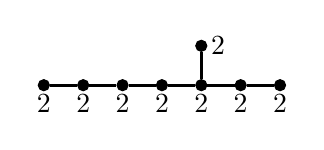
\begin{tikzpicture}
			\tikzset{dynode/.style={circle, draw, fill=black,
						minimum size=4pt, inner sep=0pt}}
			\tikzset{dyline/.style={line width=1pt}}
			\tikzset{dydash/.style={line width=1pt, dashed}}

			\begin{scope}[yshift=-10em, xshift=0]
				\node[dynode] (a1) at (0,0) {};
				\node[dynode] (a2) at (0.5,0) {};
				\node[dynode] (a3) at (1,0) {};
				\node[dynode] (a4) at (1.5,0) {};
				\node[dynode] (a5) at (2,0) {};
				\node[dynode] (a6) at (2.5,0) {};
				\node[dynode] (a7) at (3,0) {};
				\node[dynode] (a8) at (2,0.5) {};

				\draw[dyline] (a1) -- (a2) -- (a3) -- (a4) -- (a5) -- (a6) -- (a7);
				\draw[dyline] (a5) -- (a8);

				\node[below] () at (a1) {$2$};
				\node[below] () at (a2) {$2$};
				\node[below] () at (a3) {$2$};
				\node[below] () at (a4) {$2$};
				\node[below] () at (a5) {$2$};
				\node[below] () at (a6) {$2$};
				\node[below] () at (a7) {$2$};
				\node[right] () at (a8) {$2$};
			\end{scope}
		\end{tikzpicture}
		\quad\implies\quad
		\begin{pmatrix}
			2 & 1 &   &   &   &   &   &   \\
			1 & 2 & 1 &   &   &   &   &   \\
			  & 1 & 2 & 1 &   &   &   &   \\
			  &   & 1 & 2 & 1 &   &   &   \\
			  &   &   & 1 & 2 & 1 & 0 & 1 \\
			  &   &   &   & 1 & 2 & 1 & 0 \\
			  &   &   &   & 0 & 1 & 2 & 0 \\
			  &   &   &   & 1 & 0 & 0 & 2 \\
		\end{pmatrix}
	\]
	where each vertex of the tree is weighed by $2$.
\end{proposition}

It's interesting to note that if $Q$ is a matrix associated to a tree $T$, then $P(Q)$ has a $1$-skeleton homotopy equivalent to $T$. This connection between the $1$-skeleton and plumbing along a tree or graph was first noticed by Hirzebruch. It makes sense then why we'd care about matrices arising from trees instead of from general graphs which may contain cycles -- cycles break the simple-connectedness of the constructed manifold and are thereby much more complicated to work with.

% \begin{figure}[ht]\label{fig:negative-definite-trees}
% 	\centering
% 	\begin{tikzpicture}
% 		\tikzset{dynode/.style={circle, draw, fill=black,
% 					minimum size=4pt, inner sep=0pt}}
% 		\tikzset{dyline/.style={line width=1pt}}
% 		\tikzset{dydash/.style={line width=1pt, dashed}}
%
% 		\begin{scope}[yshift=0, xshift=22em]
% 			\node[dynode] (a1) at (0,0) {};
% 			\node[dynode] (a2) at (0.5,0) {};
% 			\node[dynode] (a3) at (1,0) {};
% 			\node[dynode] (a4) at (1.5,0) {};
% 			\node[dynode] (a5) at (2,0) {};
% 			\node[dynode] (a6) at (2.5,0) {};
% 			\node[dynode] (a7) at (3,0) {};
% 			\node[dynode] (a8) at (2,0.5) {};
%
% 			\draw[dyline] (a1) -- (a2) -- (a3) -- (a4) -- (a5) -- (a6) -- (a7);
% 			\draw[dyline] (a5) -- (a8);
%
% 			\node[] (l) at (1.75,-0.5) {$\E_8$};
% 		\end{scope}
%
% 		\begin{scope}[yshift=0, xshift=10em]
% 			\node[dynode] (a1) at (0,0) {};
% 			\node[dynode] (a2) at (0.5,0) {};
% 			\node[dynode] (a3) at (1,0) {};
% 			\node[dynode] (a4) at (1.5,0) {};
% 			\node[dynode] (a5) at (2,0) {};
% 			\node[dynode] (a6) at (2.5,0) {};
% 			\node[dynode] (a8) at (1.5,0.5) {};
%
% 			\draw[dyline] (a1) -- (a2) -- (a3) -- (a4) -- (a5) -- (a6);
% 			\draw[dyline] (a4) -- (a8);
%
% 			\node[] (l) at (1.5,-0.5) {$\E_7$};
% 		\end{scope}
%
% 		\begin{scope}[yshift=0, xshift=0]
% 			\node[dynode] (a1) at (0,0) {};
% 			\node[dynode] (a2) at (0.5,0) {};
% 			\node[dynode] (a3) at (1,0) {};
% 			\node[dynode] (a4) at (1.5,0) {};
% 			\node[dynode] (a5) at (2,0) {};
% 			\node[dynode] (a8) at (1,0.5) {};
%
% 			\draw[dyline] (a1) -- (a2) -- (a3) -- (a4) -- (a5);
% 			\draw[dyline] (a3) -- (a8);
%
% 			\node[] (l) at (1,-0.5) {$\E_6$};
% 		\end{scope}
%
% 		\begin{scope}[yshift=5em, xshift=3em]
% 			\node[dynode] (a1) at (0,0) {};
% 			\node[dynode] (a3) at (0.5,0) {};
% 			\node[dynode] (a4) at (1,0) {};
% 			\node[dynode] (a5) at (2.5,0) {};
% 			\node[dynode] (a6) at (3.0,0) {};
%
% 			\draw[dyline] (a1) -- (a3) -- (a4);
% 			\draw[dydash] (a4) -- (a5);
% 			\draw[dyline] (a5) -- (a6);
%
% 			\node[] (l) at (1.75,-0.5) {$\op{A}_n$};
% 		\end{scope}
%
% 		\begin{scope}[yshift=5em, xshift=17em]
% 			\node[dynode] (a1) at (0,0.4) {};
% 			\node[dynode] (a2) at (0,-0.4) {};
% 			\node[dynode] (a3) at (0.5,0) {};
% 			\node[dynode] (a4) at (1,0) {};
% 			\node[dynode] (a5) at (2.5,0) {};
% 			\node[dynode] (a6) at (3.0,0) {};
%
% 			\draw[dyline] (a1) -- (a3);
% 			\draw[dyline] (a2) -- (a3);
% 			\draw[dyline] (a3) -- (a4);
% 			\draw[dydash] (a4) -- (a5);
% 			\draw[dyline] (a5) -- (a6);
%
% 			\node[] (l) at (1.75,-0.5) {$\op{D}_n$};
% 		\end{scope}
% 	\end{tikzpicture}
% 	\vspace{1em}
% 	\caption{\todo{describe}}
% \end{figure}

\subsection{Homotopy Type of Plumbed Manifolds}



\section{Spherical Modifications}

The basic observation underlying much of surgery theory is based on the fact that for manifolds $X$ and $Y$ with boundary, we have
\[
	\partial (X\times Y) = (\partial X \times Y)\cup (X\times \partial Y).
\]
As a consequence, for integers $p,q$ the space $S^q\times S^{q-1}$ can be viewed either as the boundary of $D^{p+1}\times S^{q-1}$ or as the boundary of $S^p\times D^q$ since
\[
	\partial (S^p\times D^q) = S^p\times S^{q-1} = \partial (D^{p+1}\times S^{q-1}).
\]
Since the two products have the same boundary, whenever we find an embedding of $D^{p}\times S^{q}$ in a manifold, we can cut it out and replace it with $D^{p+1}\times S^{q-1}$.

\begin{definition}\label{def:surgery}
	Let $M$ be a smooth oriented manifold. If $f : S^q\times D^{n-q} \to M$ is a smooth embedding which maps into the interior of $M$, the \defn{surgery} of $M$ along $f$ is the smooth manifold
	\begin{equation}\label{eq:surgery-definition}
		\chi_f(M) = \left[M-\Int f(S^q\times D^{n-q})\right]\cup_{g} (D^{q+1}\times S^{n-q+1}).
	\end{equation}
	Here $g$ is the map identifying $\partial f(S^q\times D^{n-q})=f(S^q\times S^{n-q+1})$ with $\partial (D^{q+1}\times S^{n-q+1})=S^q\times S^{n-q}$.
\end{definition}

Note that $\partial (M-\Int f(S^q\times D^{n-1})) = \partial M \sqcup f(S^q\times S^{q-1})$ so $\partial \chi_f(M) = \partial M$, so surgery along an embedding into the interior does not affect the boundary.

\begin{example}\label{exam:surgery-on-a-compact-surface}
	A simple yet non-trivial example of surgery is on a surface $X_g$ of genus $g$.
	When $q=1$, note that $S^q\times D^{n-q} = S^1\times D^1$ is a cylinder, and $D^{q+1}\times S^{n-q-1}=D^2\times S^0$ is a dijsoint union of disks.
	If we embed a cylinder $S^1\times D^1$ into a ``handle'' of $X_g$, the resulting surgery cuts off this handle and reduces the genus by one. By a sequence of $g$ surgeries along embedded cylinders, we can turn $X_g$ into a sphere $X_0 = S^2$.
	\begin{figure}[ht]
		\centering
		\import{graphics/temp-diagrams/}{surgery-on-two-holed-torus.pdf_tex}
		\caption{Turning a genus 2 surface into a genus 1 surface via surgery.}\label{fig:surgery-on-two-holed-torus}
	\end{figure}
\end{example}

\begin{remark}
	Technically, the result of \cref{eq:surgery-definition} does not have an a priori smooth structure at the gluing set $f(S^q\times S^{n-q+1})$.
	\todo{smoothing out the corners.}
\end{remark}

While surgery clearly alters the topology of a manifold, it preserves the cobordism type.
\begin{definition}
	The \defn{trace}[trace of a surgery] $W_f(M)$ of a surgery $\chi_f(M)$ is the space
	\[
		W_f(M) = (D^{q+1}\times D^{n-q})\cup_h (M\times I)
	\]
	where $h$ is the map identifying $\partial D^{q+1}\times D^{n-q}$ with $f(S^q\times D^{n-q})\times \{1\}$.
\end{definition}

Note that $\partial W_f(M) = \chi_f(M) \sqcup (-M)$, so $W_f(M)$ is a cobordism $\chi_f(M) \bord M$. Consequently, surgery does not affect the cobordism type of a manifold and can thus be used to find a simplest representative for a given cobordism class.

\todo{finish this section}

\section{Framed Surgery}

\begin{definition}
	A \defn{framed manifold} is a pair $(M, F)$ consisting of a manifold $M$ and a \defn{framing}[framing of a manifold] $F$ which is a trivialization of the stable tangent bundle $\T M \oplus\underline{\R}^q$ for some $q>0$.
\end{definition}

\begin{definition}
	A \defn{framed cobordism} is
\end{definition}

\begin{theorem}
	Let $W$ be a compact framed manifold of dimension $n\geq 4$ such that the boundary $\partial W$ is a homology sphere. By a sequence of framed surgeries, $W$ can be made $\lfloor\frac{n-1}{2}\rfloor$-connected.
\end{theorem}

\begin{corollary}
	For any $k\geq 2$, we have $\bP^{2k+1}=0$.
\end{corollary}

\todo{finish this section}


\subsection{The Plumbing Theorem}\label{sec:plumbing-theorem}

\begin{proposition}
	If $\partial P^{2m}(Q)$ is a homotopy sphere then $Q$ is unimodular.
\end{proposition}

\begin{theorem}
	When $k>1$, $\partial P^{4k}(Q)$ is a homotopy sphere if and only if $Q$ is unimodular.
\end{theorem}


\begin{proposition}
	The signature of a highly-connected $4k$-dimensional manifold boundary empty or a homotopy sphere is divisible by $8$.
\end{proposition}

\begin{definition}
	For $k>1$, the \defn{Milnor sphere} is the homotopy sphere $\partial P^{4k}(E_8)$.
\end{definition}

\begin{definition}
	\todo{normal map}
\end{definition}

\begin{definition}
	\todo{surgical invariant $\sigma$}
\end{definition}

\begin{theorem}[Plumbing Theorem]\label{thm:plumbing-theorem}
	When $m>2$, there is a normal map \[(g,c) : (W,\partial W) \to (D^{2m}, S^{2m-1})\] which restricts to a homotopy equivalence $g|_{\partial W} : \partial W \to  S^{2m-1}$ with the invariant $\sigma(g,c)$ taking on any integer value.
\end{theorem}

\subsection{Surgery Theory in General}
\todo{general exact sequence}
\[
	L_{n+1}(\Z[\pi_1(X)]) \lkxto \mathcal{S}^\DIFF(X) \lkxto {[X, G/\DIFF]} \lkxto L_n(\Z[\pi_1(X)])
\]

